
\documentclass{article}
% pre\'ambulo

\usepackage{lmodern}
\usepackage[T1]{fontenc}
\usepackage[spanish,activeacute]{babel}
\usepackage{enumerate}
\usepackage{graphicx}
\graphicspath{ {/home/nestor2502/Modelado/Tarea01/imagenes/} }

\title{Tarea 01}
\author{Nestor Semer V\'azquez Cordero}
\date{14 de Agosto del a\~no 2019}

\begin{document}
% cuerpo del documento

\maketitle

\section{Definici\'on del problema}

Dar el clima en tiempo real de dos localidades dadas su latitud y longitud, 
usando un web service para poder realizar las multiples peticiones que se requieren.

\section{Analisis del problema}
Se tiene que procesar un archivo .csv el cual contiene en cada rengl\'on: ciudad de origen, 
ciudad de destino, latitud origen, longitud de origen, latitud de destino y longitud de destino;
los datos deben ser proporcionados por el usuario, esos datos son suficientes para poder obtener el clima 
de un web service.

Debido a que son multiples peticiones al servidor, se utilizar\'an hilos de ejcucion en cada petici\'on
asi disminuir dr\'asticamente el tiempo de ejecucion en comparaci\'on a un programa que no
utilice hilos de ejecucion.

Como todo programa es propenso a errores, hay que intentar disminuirlos
para que al momento de que el usuario ejecute el programa no salte una excepci\'on, para eso se necesita resolver varios problemas, en este programa se considerar\'an los siguientes:

\begin{itemize}
 \item El servidor no est\'a disponible
 \item No hay conexi\'on a internet
 \item No se encuentra el archivo en la ruta indicada
 \item El archivo no tiene el formato .csv
 \item No se especifica la ciudad
 \item No se especifica latitud ni longitud
 \end{itemize}

\section{Seccion de la mejor alternativa}

Se utilizar\'a el lenguaje de programacio\'n python ya que es un lenguaje 
lenguaje de alto nivel, 
debido a eso la sintaxis es sencilla de aprender en poco tiempo, adem\'as  hay librerias que facilitan
el trabajo, la biblioteca que se usar\'a es ''request'' el cual nos 
permitir\'a realizar las peticiones y obtener un json, el cual contendr\'a la informacion que requerimos.
El web service que se utilizar\'a es open weather ya que es el mas sencillo de manejar, adem\'as la documentacion
que se encuentra en la p\'agina es muy completa.
Nota:El numero maximo de peticiones que nos permite de manera gratuita el 
servidor seleccionado es de 60 peticiones por minuto, si se excede el numero maximo de peticiones
se bloquea la cuenta y por consecuencia no permite realizar peticiones. 

\section{Diagrama de flujo }

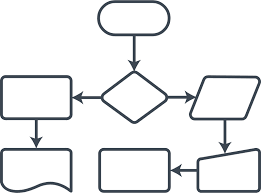
\includegraphics{diagrama}

\section{Pensando en el futuro}

Para este punto se piensa realizar una funci\'on que \'unicamente
reciba como parametros latitud y longitud, as\'i se puede modificar el servidor, ya sea para cambiar la informacion que se muestra al 
usuario y esta sea mas acorde a sus necesidades o cambiar de proveedor de servicios web si el cliente asi lo desea.


Por ultimo, creo que cobrar\'ia cerca de \$1000 por el tiempo dedicado, adem\'as se gantiza que el programa realizar\'a exactamente lo que se plante\'o en la definicion del problema.

\end{document}
